%%%%%%%%%%%%%%%%%%%%%%%%%%%%%%%%%%%%% BEGIN HEADERS %%%%%%%%%%%%%%%%%%%%%%%%%%%%%%%%%%%%%%%%%%%%%%%%%%%%%
\documentclass[11pt,conference]{IEEEtran}

\usepackage{longtable}
\usepackage{graphicx}
\usepackage[utf8]{inputenc}
\usepackage{fancyhdr}
\usepackage{float}
\usepackage[hidelinks]{hyperref}
\usepackage{listings}
\usepackage{color}
\usepackage{natbib}

% Your names in the header
\pagestyle{fancy}
\rhead{Enrico Tedeschi}
\lhead{INF-3201 Parallel Programming - Assignment 2}
\cfoot{\thepage}

% Used for including code in a stylized manner
\definecolor{codegreen}{rgb}{0,0.6,0}
\definecolor{codegray}{rgb}{0.5,0.5,0.5}
\definecolor{codepurple}{rgb}{0.58,0,0.82}
\definecolor{backcolour}{rgb}{0.95,0.95,0.92}
 

\lstdefinestyle{mystyle}{
    backgroundcolor=\color{backcolour},   
    commentstyle=\color{codegreen},
    keywordstyle=\color{magenta},
    numberstyle=\tiny\color{codegray},
    stringstyle=\color{codepurple},
    basicstyle=\footnotesize,
    breakatwhitespace=false,         
    breaklines=true,                 
    captionpos=b,                    
    keepspaces=true,                 
    numbers=left,                    
    numbersep=5pt,                  
    showspaces=false,                
    showstringspaces=false,
    showtabs=false,                  
    tabsize=2
}

\lstset{style=mystyle}

% The Title
\title{INF-3201 Parallel Programming
\newline
Shared Memory}

% Your name and email
\author{\textbf{Enrico Tedeschi}\\ ete011@post.uit.no }


%%%%%%%%%%%%%%%%%%%%%%%%%%%%%%%%%%%%% END HEADERS %%%%%%%%%%%%%%%%%%%%%%%%%%%%%%%%%%%%%%%%%%%%%%%%%%%%%

\begin{document}

% Create the title and everything
\maketitle

\section{Introduction}
The goal of this assignment is to parallelize a piece of code using shared memory techniques preferably using \textbf{OpenMP}.
\subsection{Requirements}
\begin{itemize} 
\item Choose a piece of software to parallelize
\item Parallelize it with shared-memory techniques
\item Evaluate speedup
\end{itemize}


\section{Technical Background}

\begin{itemize} 
\item[--] Concurrency and parallelism concepts
\item[--] Parallel programming concepts
\item[--] Basic programming approach
\item[--] Knowledge of C language
\item[--] Notion of design pattern principles
\item[--] Theory about software engineering
\item[--] Knowledge of git to manage the software versions
\end{itemize}


\section{Analysis}
The given \textbf{Markovian} code was found to be too long and quite hard to understand, in addition, it has no deterministic solution so it would have been really difficult to test.
\newline
The code chosen to be parallelized is a sequential version of the \textbf{TSP} (Traveller Salesman Problem). It asks the following question: \textit{Given a list of cities and the distances between each pair of cities, what is the shortest possible route that visits each city exactly once and returns to the origin city?} \cite{citation1}
\newline
The sequential code was refined by adding a random function which generate distances between cities and also the possibility of run the programme with a size passed as a parameter was implemented.
\newline
To parallelize a sequential code is necessary to analyse which function involves the biggest amount of time. The c given program \textit{tsp-seq.c} has been tested with \textit{profile} and the following table is the result of this test:
\begin{lstlisting}
  %   cumulative   self               
 time   seconds    calls   name    
100.32   2.90        1     zRoute
  0.00   0.00      196     zEuclidDist
  0.00   0.00       28     random_at_most
  0.00   0.00        2     second
  0.00   0.00        1     zReadRoute
\end{lstlisting}

the function to parallelize is obviously \textit{zRoute}.
\newline
The function has a recursive structure for each possible successor of the city chosen as initial. For instance, if the function would have a $iSize = 5$ (number of cities) then the execution tree would look like the one in Fig \ref{fig:tree}. 
In the first 'level' of the tree the first city executes recursively the $zRoute$ function for the number of the cities left to visit, and so for the other levels.
Having an image of the execution tree helps to get the parallelization easier.
\begin{figure}[h!]
  \centering
    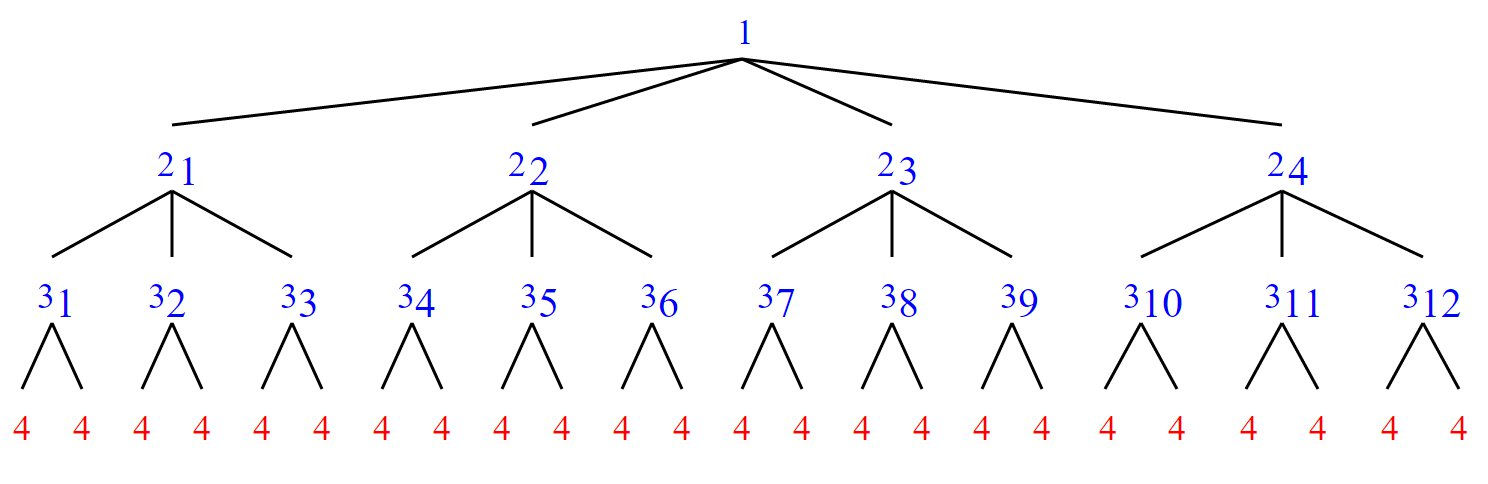
\includegraphics[width=0.5\textwidth]{tree}
    \caption{Execution of the zRoute function}
    \label{fig:tree}
\end{figure}

\section{Implementation}
%TODO: talk about random function, and parameters in input
%TODO: draw the parallelized tree
%TODO: how achieve the parallelization with openMP
\subsection{Environment}
\subsection{}

\section{Result and Benchmarking}
%TODO: scale with number of cities
%TODO: compare with the sequential one


\section{Discussion}



\section{Conclusion}

\bibliographystyle{plain}
\bibliography{report}


\end{document}

